\documentclass{article}
\usepackage{amsmath}
\usepackage[mathletters]{ucs}
\usepackage[utf8x]{inputenc}
\usepackage[margin=1.5in]{geometry}
\usepackage{enumerate}
\newtheorem{theorem}{Theorem}
\usepackage[dvipsnames]{xcolor}
\usepackage{pgfplots}
\setlength{\parindent}{0cm}
\usepackage{graphics}
\usepackage{graphicx} % Required for including images
\usepackage{subcaption}
\usepackage{bigintcalc}
\usepackage{pythonhighlight} %for pythonkode \begin{python}   \end{python}
\usepackage{appendix}
\usepackage{arydshln}
\usepackage{physics}
\usepackage{tikz-cd}
\usepackage{booktabs} 
\usepackage{adjustbox}
\usepackage{mdframed}
\usepackage{relsize}
\usepackage{physics}
\usepackage[thinc]{esdiff}
\usepackage{fixltx2e}
\usepackage{esint}  %for lukket-linje-integral
\usepackage{xfrac} %for sfrac
\usepackage{hyperref} %for linker, må ha med hypersetup
\usepackage[noabbrev, nameinlink]{cleveref} % to be loaded after hyperref
\usepackage{amssymb} %\mathbb{R} for reelle tall, \mathcal{B} for "matte"-font
\usepackage{listings} %for kode/lstlisting
\usepackage{verbatim}
\usepackage{graphicx,wrapfig,lipsum,caption} %for wrapping av bilder
\usepackage{mathtools} %for \abs{x}
\usepackage[norsk]{babel}
\definecolor{codegreen}{rgb}{0,0.6,0}
\definecolor{codegray}{rgb}{0.5,0.5,0.5}
\definecolor{codepurple}{rgb}{0.58,0,0.82}
\definecolor{backcolour}{rgb}{0.95,0.95,0.92}
\lstdefinestyle{mystyle}{
    backgroundcolor=\color{backcolour},   
    commentstyle=\color{codegreen},
    keywordstyle=\color{magenta},
    numberstyle=\tiny\color{codegray},
    stringstyle=\color{codepurple},
    basicstyle=\ttfamily\footnotesize,
    breakatwhitespace=false,         
    breaklines=true,                 
    captionpos=b,                    
    keepspaces=true,                 
    numbers=left,                    
    numbersep=5pt,                  
    showspaces=false,                
    showstringspaces=false,
    showtabs=false,                  
    tabsize=2
}

\lstset{style=mystyle}
\author{Oskar Idland}
\title{Problem Set 1}
\date{}
\begin{document}
\maketitle
\newpage

\section*{Problem 1.1 (L)}
We define $ \ket{u}$ and $ \bra{u}$. 
\[
\ket{u} = α \ket{u_1} + β \ket{u_2} \quad , \quad \bra{u} = \ket{u}^{†} = α^* \bra{u_1} + β^* \bra{u_2}
\]

Using the distributive property of the inner product, we get
\[
\bra{u}\ket{w} = \left(α^{*} \bra{u_1} + β^{*} \bra{u_2} \right) \ket{w} = α^{*} \bra{u_1}\ket{w} + β^{*} \bra{u_2}\ket{w}
\]

\section*{Problem 1.2 (L)}
Defining $ \ket{w}$. 
\[
\ket{w} = α \ket{w_1} + β \ket{w_2} 
\]
Defining the relationship between $ \ket{w}$ and $ \bra{w}$.
\[
\bra{w} = \ket{w}^{†} = \left(α \ket{w_1} + β \ket{w_2}\right) ^{†}
\]
Using the distributive property of the conjugate transpose, we arrive at
\[
\bra{w} = \left(α \ket{w_1}\right)^{†} + \left(β \ket{w_2}\right)^{†} = α^{*} \bra{w_1} + β^{*} \bra{w_2}
\]

\section*{Problem 1.3 (L)}
\[
\bra{f}\ket{g} = ∫_{a}^{b} f(x)^{*} g(x) \ \mathrm{d}x
\]
\[
\bra{f}\ket{f} = ∫_{a}^{b} f(x)^2 \ \mathrm{d}x
\]

All values of $f(x)^2$ are greater or equal to zero. Therefore, the integral is only zero if $f(x) = 0$ for all $x$.  

\section*{Problem 1.4 (L)}
\[
\bra{a_i}\ket{V} = ∑_{j=1}^{N} \bra{a_i}v_i \ket{a_j}
\]
As all the basis vectors are orthonormal, the only non-zero term in the sum is when $i = j$. As the basis vectors are orthonormal their magnitude is one. Therefore, we get the following. 
\[
v_i \bra{a_i}\ket{a_i} = v_i 
\]

\section*{Problem 1.5 (L)}
\[
\bra{x}\ket{f} = ∫ dx' f(x') \bra{x}\ket{x'} = ∫ dx' f(x') δ(x-x')
\]
The Dirac delta picks out the only value of $x'$ that gives a non-zero value. Therefore, we get the following.
\[
∴ \bra{x}\ket{f} = f(x)
\]

Applying the identity $\mathbf{I}$ operator to $ \ket{f}$, we get the following.

\[
\mathbf{I} \ket{x} = ∫_{0}^{L}\mathrm{d}x' \ket{x'} \bra{x'} \ket{x} = ∫_{0}^{L}\mathrm{d}x' \ket{x'} δ(x-x') = \ket{x} 
\]

\section*{Problem 1.6 (H)}
\subsection*{a)}
Using trig identities we know that
\[
∫_{-∞}^{∞} δ_{ϵ}(x) \ \mathrm{d}x = \frac{1}{π} \left[\arctan (x / ϵ)\right]_{-∞}^{∞} = \frac{1}{π} \left[\frac{π}{2} - \left(-\frac{π}{2}\right)\right] = 1
\]
\subsection*{b)}
\[
δ_{ϵ / k}(x) = k δ_{ϵ}(kx)
\]
\[
\frac{1}{kπ} \frac{ϵ}{ϵ^2 + x^2} = \frac{k}{π} \frac{ϵ}{ϵ^2 + (kx)^2} 
\]
\[
\frac{1}{kπ} \frac{ϵ}{ϵ^2 + x^2} = \frac{k}{k^2π} \frac{ϵ}{ϵ^2 + x^2} = \underline{\underline{\frac{1}{kπ} \frac{ϵ}{ϵ^2 + x^2}}} 
\]
\newpage
\subsection*{c)}
\begin{figure}[h!]
  \centering
  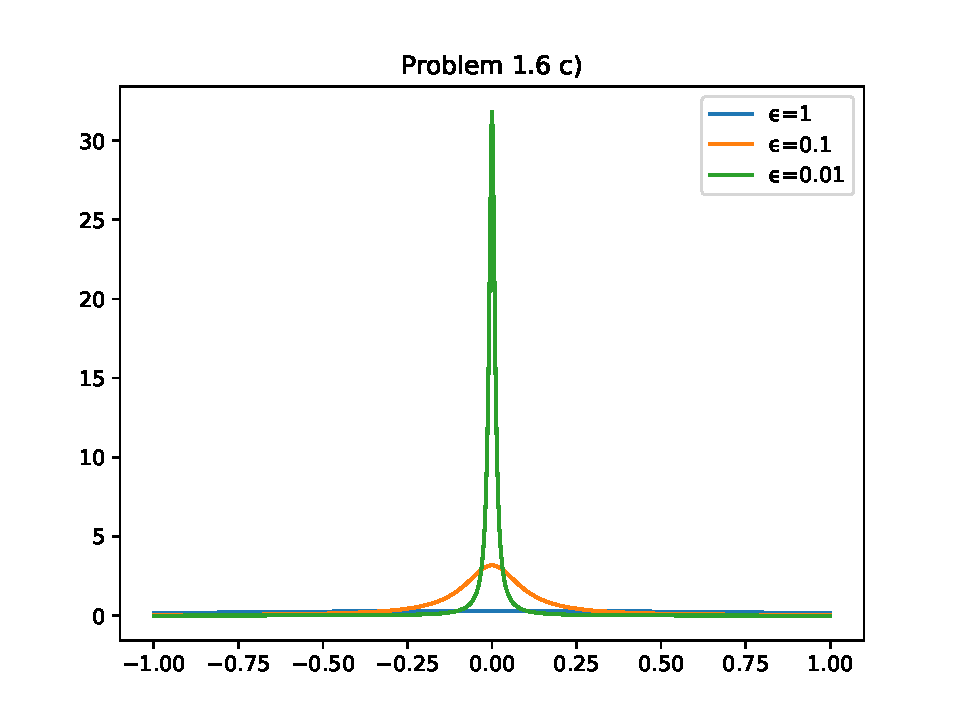
\includegraphics[width = \textwidth]{E_1.6.pdf}
  \caption{Numerical plot of $δ_{ϵ}(x)$ for $ϵ = 1$, $ϵ = 0.1$ and $ϵ = 0.01$.}
  \label{fig: }
\end{figure}

\section*{d)}
Assuming we have an infinite number of arguments $x$ and values $y = δ_1(x)$, we can use the conclusions from exercise b). 
\[
δ_{0.1}(x) = 10 δ_{1}(10x).  
\]
To obtain a similar table for the new function $δ_{0.1}$(x), we map our new table's $y$-value to the table of $δ_1$ $y$-value for the same $x$-argument times 10, and multiply that result again, by 10. 

\[
x_{0.1} ↦ x_1 \quad , \quad y_{0.1} ↦ 10 y_1(10 x_1)
\]


\section*{Problem 1.7 (H)}
As the basis are orthonormal we know $ \bra{b_i}\ket{b_j} = 1$, if $i = j$. 
\[
\hat{P}_1 \ket{A} = ∑_{i=1}^{N} \ket{b_1} \bra{b_1} α_i \ket{b_i} = \underline{\underline{α_1 \ket{b_1}}}
\]
\[
\hat{P}_1 \hat{P}_1 \ket{A} = \hat{P}_1 α_1 \ket{b_1} = α_1 \ket{b_1} \underbrace{\bra{b_1}\ket{b_1}}_{1} = \underline{\underline{α_1 \ket{b_1}}}
\]

The operator $\hat{P}_1$ can be considered as a projection operator. It finds the projection of the ket $\ket{A}$ onto the basis vector $\ket{b_1}$. As the basis vectors are orthonormal, the operator $\hat{P}_1$ only picks out the component of $\ket{A}$ that is parallel to $\ket{b_1}$ together with its magnitude. 

\section*{Problem 1.8 (E)}
A quantum state is a complex vector (ket) in a Hilbert space. The ket vector contains all there is to know about the system. It contains the probabilities of all possible outcomes of a measurement. The difference between a quantum state and a classical state, is that the classical state does not change when measured, but the quantum state does. With a complete description of a classical state you know deterministically how it will behave in the past and future. With a quantum state it's only probabilistic what might happen in the future. To gather information of a classical state, you just need to look at the values. Its position is just its position. To gather information of a quantum state, we use operators, which acts on the ket, and gives us the probabilities of different outcomes.  

\section*{Problem 1.9 (E)}
\[
\ket{u} ≃ \begin{pmatrix*}[r]
 u_1 \\
 u_2 \\
\end{pmatrix*} \quad , \quad 
\ket{v} ≃ \begin{pmatrix*}[r]
 v_1 \\
 v_2 \\
\end{pmatrix*} \quad , \quad 
α = a + ib
\]
\[
\bra{u}\ket{v} = \underline{\underline{u_1 v_1 + u_2 v_2}}
\]
\[
\bra{u}α \ket{v} = \bra{u} \left(a\ket{v} + ib\ket{v}\right) = a \bra{u}\ket{v} + ib \bra{u}\ket{v}
\]
\[
\bra{u}α \ket{v} = \underline{\underline{au_1v_1 + ibu_2v_2}}
\]
\end{document}